%% arrowLength=20
%% linkWidth=2
%% input fy=50*node.pos
%% output fx=700
%% output fy=150*node.pos+120
%% MAX_FONT_SIZE=12
\begin{table}[H]
    \begin{center}
        \begin{tabular}{||l c c c||}
            \hline
            & 1      & 2      & 3 \\ [0.5ex]
            \hline
            velikost populacije               & 200    & 250    & 350    \\
            \hline
            največje število globokih vozlišč & 15     & 20     & 25     \\
            \hline
            največje število povezav          & 30     & 50     & 75     \\
            \hline
            največje število prečkanj         & 2      & 3      & 4      \\
            \hline
            delež mutiranih potomcev          & 10\%   & 10\%   & 10\%   \\
            \hline
            prispevek vozlišč                 & -0.001 & -0.001 & -0.001 \\
            \hline
            prispevek povezav                 & -0.001 & -0.001 & -0.001 \\
            \hline
            število generacij                 & 300    & 350    & 450    \\
            \hline
        \end{tabular}
    \end{center}
    \caption{Nabori inicializacijskih parametrov poganjanja na množici Wine.}
    \label{tab:param_wine}
\end{table}

\subsection{Prvi nabor}\label{subsec:dodatek-wine-prvi-nabor}
%%"/home/jure/CLionProjects/Neuroevolution/datasets/wine/wine.data" 200 15 30 2 true 0.1 100 true -0.001 -0.001 300 ACC
\begin{table}[H]
    \begin{center}
        \begin{tabular}{|| c | c c || c c ||}
            \hline
            \multirow{2}{*}{št. zagona} & \multicolumn{2}{c||}{točnost najboljšega agenta} & \multicolumn{2}{c||}{MCC najboljšega agenta} \\ \cline{2-5}
            & učna   & testna          & učna  & testna                  \\
            \hline
            1        & 92.0\% & 75.5\%          & 0.868 & \textbf{0.918 (94.3\%)} \\
            \hline
            2        & 94.4\% & 92.5\%          & 0.808 & 0.843                   \\
            \hline
            3        & 92.0\% & 92.5\%          & 0.818 & 0.779                   \\
            \hline
            4        & 96.8\% & \textbf{94.3\%} & 0.820 & 0.677                   \\
            \hline
            5        & 84.8\% & 75.5\%          & 0.904 & 0.830                   \\
            \hline
            $\sigma$ & 0.040  & 0.086           & 0.037 & 0.08                    \\
            \hline
        \end{tabular}
    \end{center}
    \caption{Rezultat prvega nabora parametrov.}
    \label{tab:wine_result_1}
\end{table}

\begin{table}[H]
    \centering
    \begin{tabular}{||rcccc||}
        \hline
        razred  & Class 1 & Class 2 & Class 3 & vsota \\ \hline
        Class 1 & 17      & 1       & 0       & 18    \\ \hline
        Class 2 & 2       & 19      & 0       & 21    \\ \hline
        Class 3 & 0       & 0       & 14      & 14    \\ \hline
        vsota   & 19      & 20      & 14      & 53    \\ \hline
    \end{tabular}
    \caption{Matrika zmot najbolj točnega agenta prvega nabora.}
    \label{tab:wine_acc_1}
\end{table}

\begin{table}[H]
    \centering
    \begin{tabular}{||rcccc||}
        \hline
        razred  & Class 1 & Class 2 & Class 3 & vsota \\ \hline
        Class 1 & 18      & 0       & 0       & 18    \\ \hline
        Class 2 & 2       & 18      & 1       & 21    \\ \hline
        Class 3 & 0       & 0       & 14      & 14    \\ \hline
        vsota   & 20      & 18      & 15      & 53    \\ \hline
    \end{tabular}
    \caption{Matrika zmot agenta z največjim MCC prvega nabora.}
    \label{tab:wine_mcc_1}
\end{table}

\begin{figure}[H]
    \begin{center}
        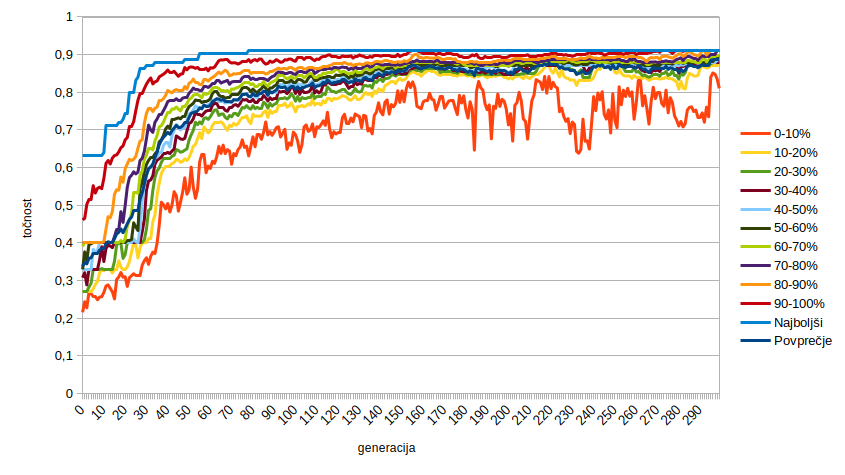
\includegraphics[width=13cm]{wine/1/acc}
    \end{center}
    \caption{Graf točnosti populacije najboljšega agenta prvega nabora skozi generacije.}
    \label{fig:wine_acc_1}
\end{figure}

\begin{figure}[H]
    \begin{center}
        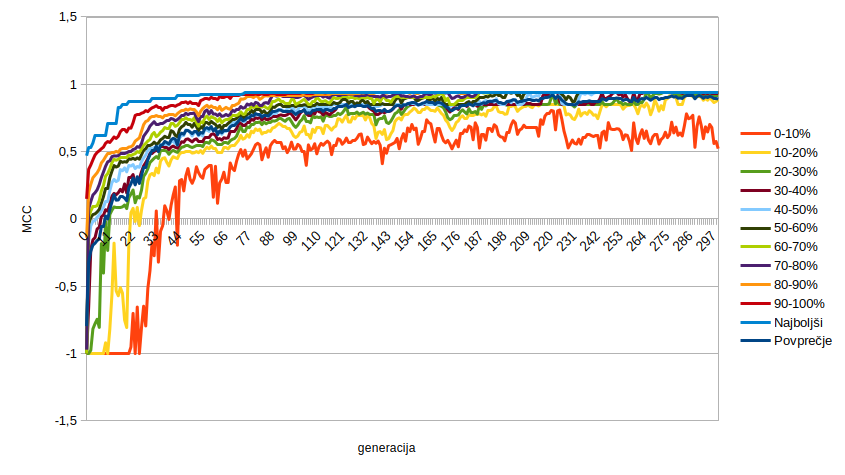
\includegraphics[width=13cm]{wine/1/mcc}
    \end{center}
    \caption{Graf MCC populacije najboljšega agenta prvega nabora skozi generacije.}
    \label{fig:wine_mcc_1}
\end{figure}

\begin{figure}[H]
    \begin{center}
        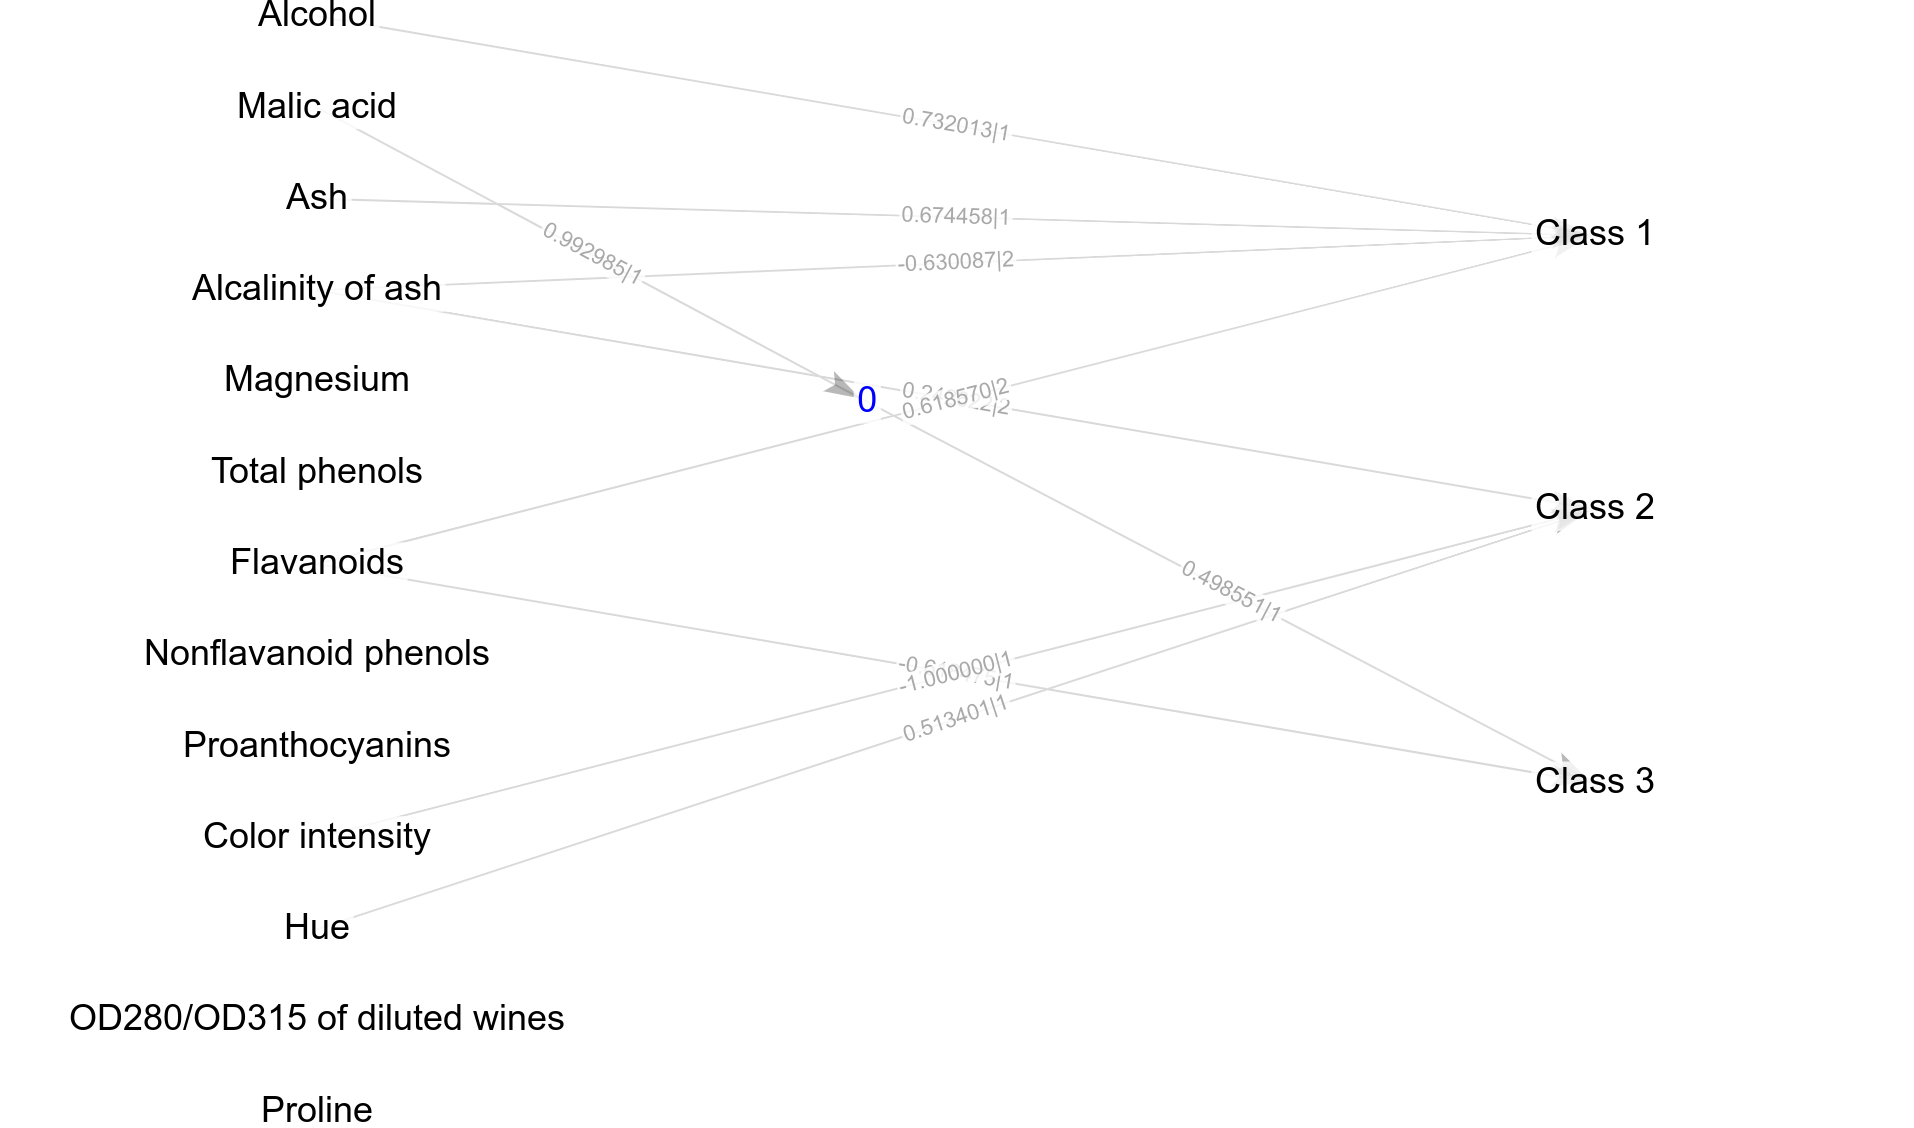
\includegraphics[width=13cm]{wine/1/acc_g}
    \end{center}
    \caption{Vizualizacija najbolj točnega agenta prvega nabora. Vsebuje 1 globoko vozlišče in 9 povezav.}
    \label{fig:wine_acc_1_g}
\end{figure}

\begin{figure}[H]
    \begin{center}
        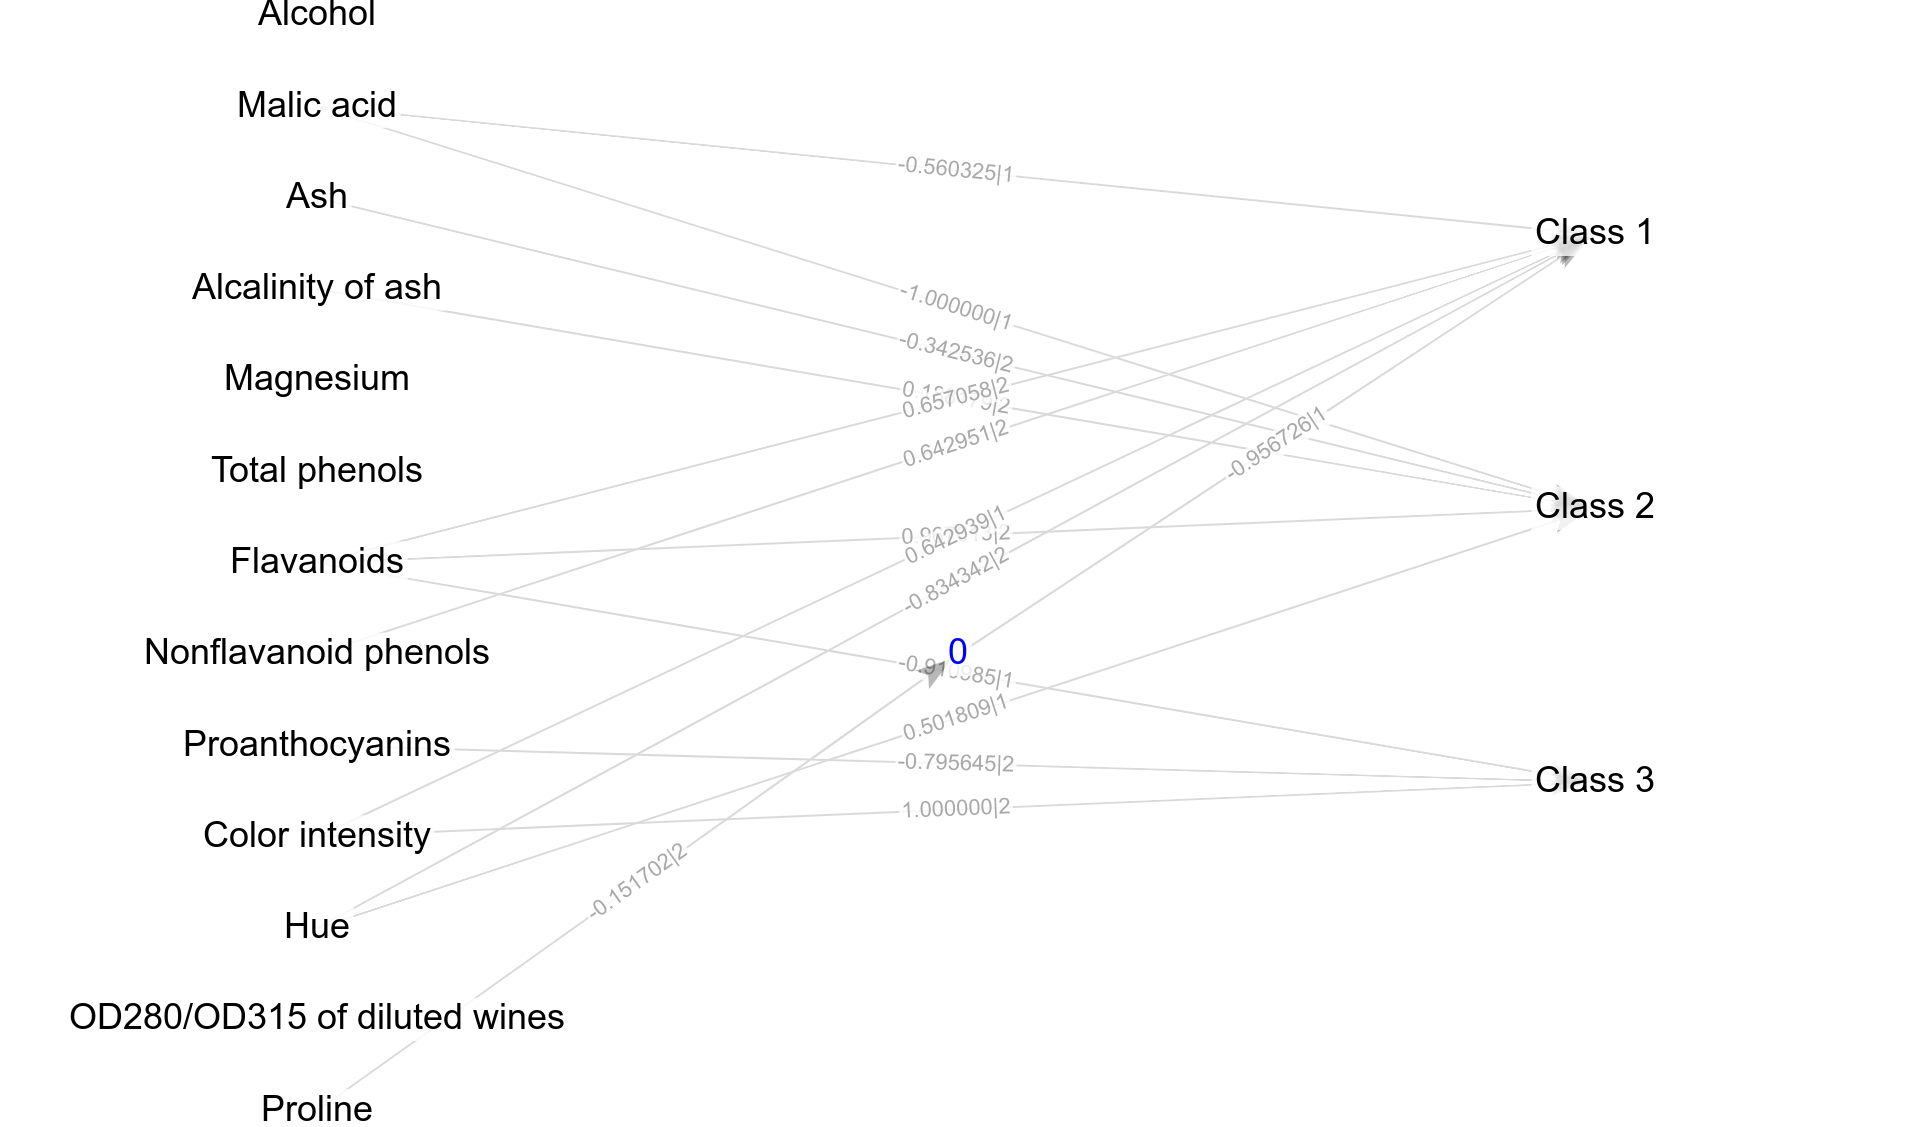
\includegraphics[width=13cm]{wine/1/mcc_g}
    \end{center}
    \caption{Vizualizacija agenta z največjim MCC prvega nabora. Vsebuje 6 povezav.}
    \label{fig:wine_mcc_1_g}
\end{figure}

\subsection{Drugi nabor}\label{subsec:dodatek-wine-drugi-nabor}
%%"/home/jure/CLionProjects/Neuroevolution/datasets/iris/iris.data" 250 20 50 3 true 0.1 100 true -0.001 -0.001 350 ACC
\begin{table}[H]
    \begin{center}
        \begin{tabular}{|| c | c c || c c ||}
            \hline
            \multirow{2}{*}{št. zagona} & \multicolumn{2}{c||}{točnost najboljšega agenta} & \multicolumn{2}{c||}{MCC najboljšega agenta} \\ \cline{2-5}
            & učna   & testna          & učna  & testna                  \\
            \hline
            1        & 83.2\% & 81.1\%          & 0.845 & 0.610                   \\
            \hline
            2        & 67.2\% & 60.4\%          & 0.867 & 0.779                   \\
            \hline
            3        & 76.8\% & 77.4\%          & 0.830 & 0.740                   \\
            \hline
            4        & 92.0\% & \textbf{96.2\%} & 0.915 & \textbf{0.915 (94.3\%)} \\
            \hline
            5        & 93.6\% & 96.2\%          & 0.892 & 0.914                   \\
            \hline
            $\sigma$ & 0.098  & 0.134           & 0.031 & 0.115                   \\
            \hline
        \end{tabular}
    \end{center}
    \caption{Rezultat drugega nabora parametrov.}
    \label{tab:wine_result_2}
\end{table}

\begin{table}[H]
    \centering
    \begin{tabular}{||rcccc||}
        \hline
        razred  & Class 1 & Class 2 & Class 3 & vsota \\ \hline
        Class 1 & 17      & 1       & 0       & 18    \\ \hline
        Class 2 & 0       & 20      & 1       & 21    \\ \hline
        Class 3 & 0       & 0       & 14      & 14    \\ \hline
        vsota   & 17      & 21      & 15      & 53    \\ \hline
    \end{tabular}
    \caption{Matrika zmot najbolj točnega agenta drugega nabora.}
    \label{tab:wine_acc_2}
\end{table}

\begin{table}[H]
    \centering
    \begin{tabular}{||rcccc||}
        \hline
        razred  & Class 1 & Class 2 & Class 3 & vsota \\ \hline
        Class 1 & 17      & 1       & 0       & 18    \\ \hline
        Class 2 & 2       & 19      & 0       & 21    \\ \hline
        Class 3 & 0       & 0       & 14      & 14    \\ \hline
        vsota   & 19      & 20      & 14      & 53    \\ \hline
    \end{tabular}
    \caption{Matrika zmot agenta z največjim MCC drugega nabora.}
    \label{tab:wine_mcc_2}
\end{table}

\begin{figure}[H]
    \begin{center}
        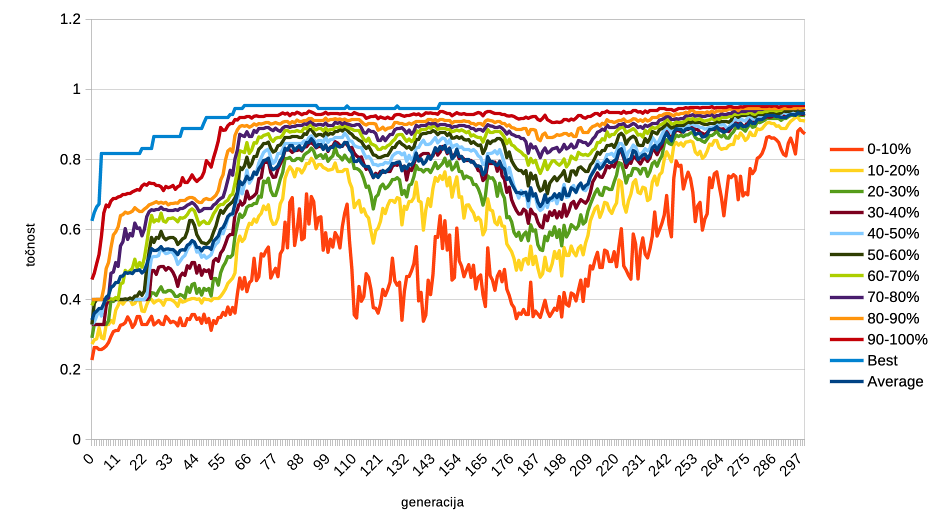
\includegraphics[width=13cm]{wine/2/acc}
    \end{center}
    \caption{Graf točnosti populacije najboljšega agenta drugega nabora skozi generacije.}
    \label{fig:wine_acc_2}
\end{figure}

\begin{figure}[H]
    \begin{center}
        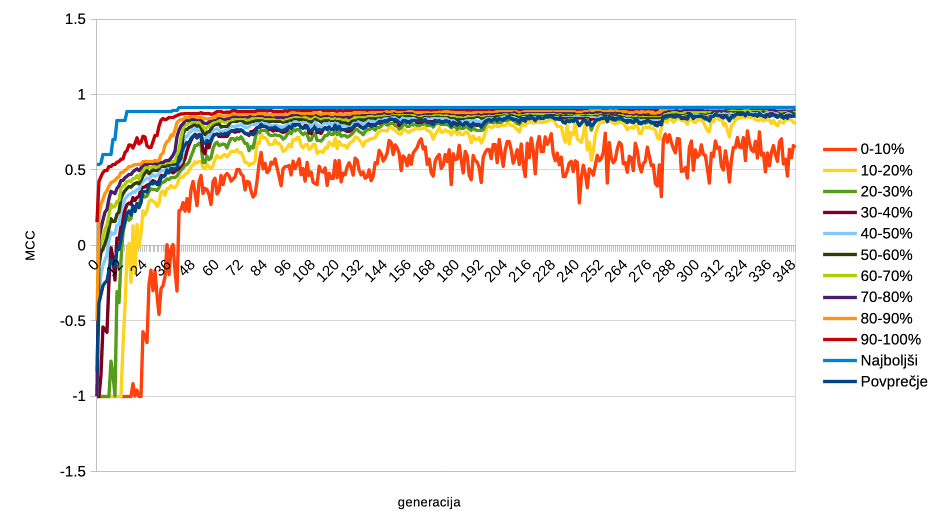
\includegraphics[width=13cm]{wine/2/mcc}
    \end{center}
    \caption{Graf MCC populacije najboljšega agenta drugega nabora skozi generacije.}
    \label{fig:wine_mcc_2}
\end{figure}

\begin{figure}[H]
    \begin{center}
        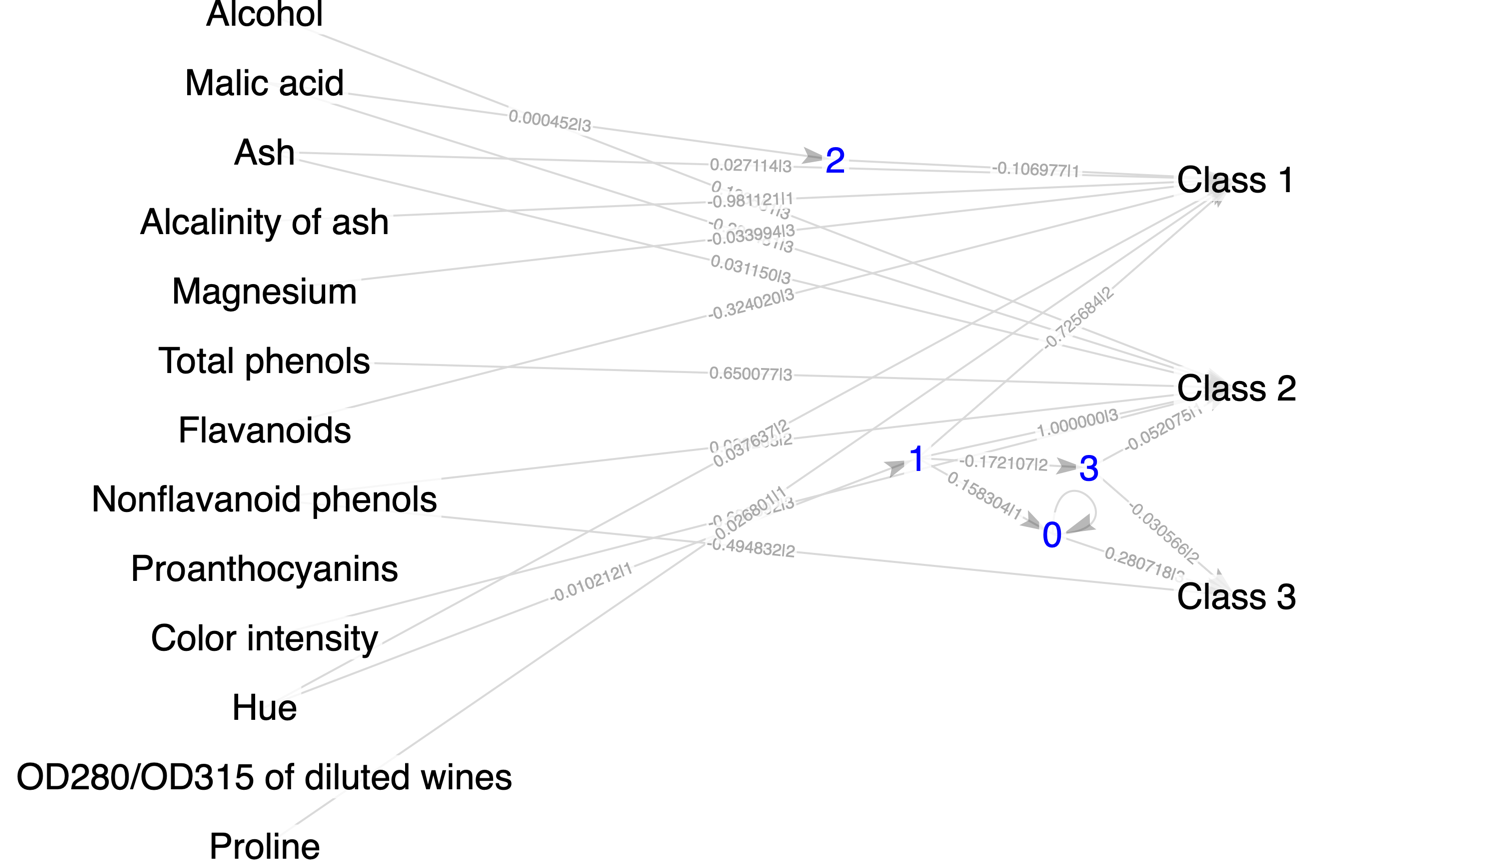
\includegraphics[width=13cm]{wine/2/acc_g}
    \end{center}
    \caption{Vizualizacija najbolj točnega agenta drugega nabora. Vsebuje 6 povezav.}
    \label{fig:wine_acc_2_g}
\end{figure}

\begin{figure}[H]
    \begin{center}
        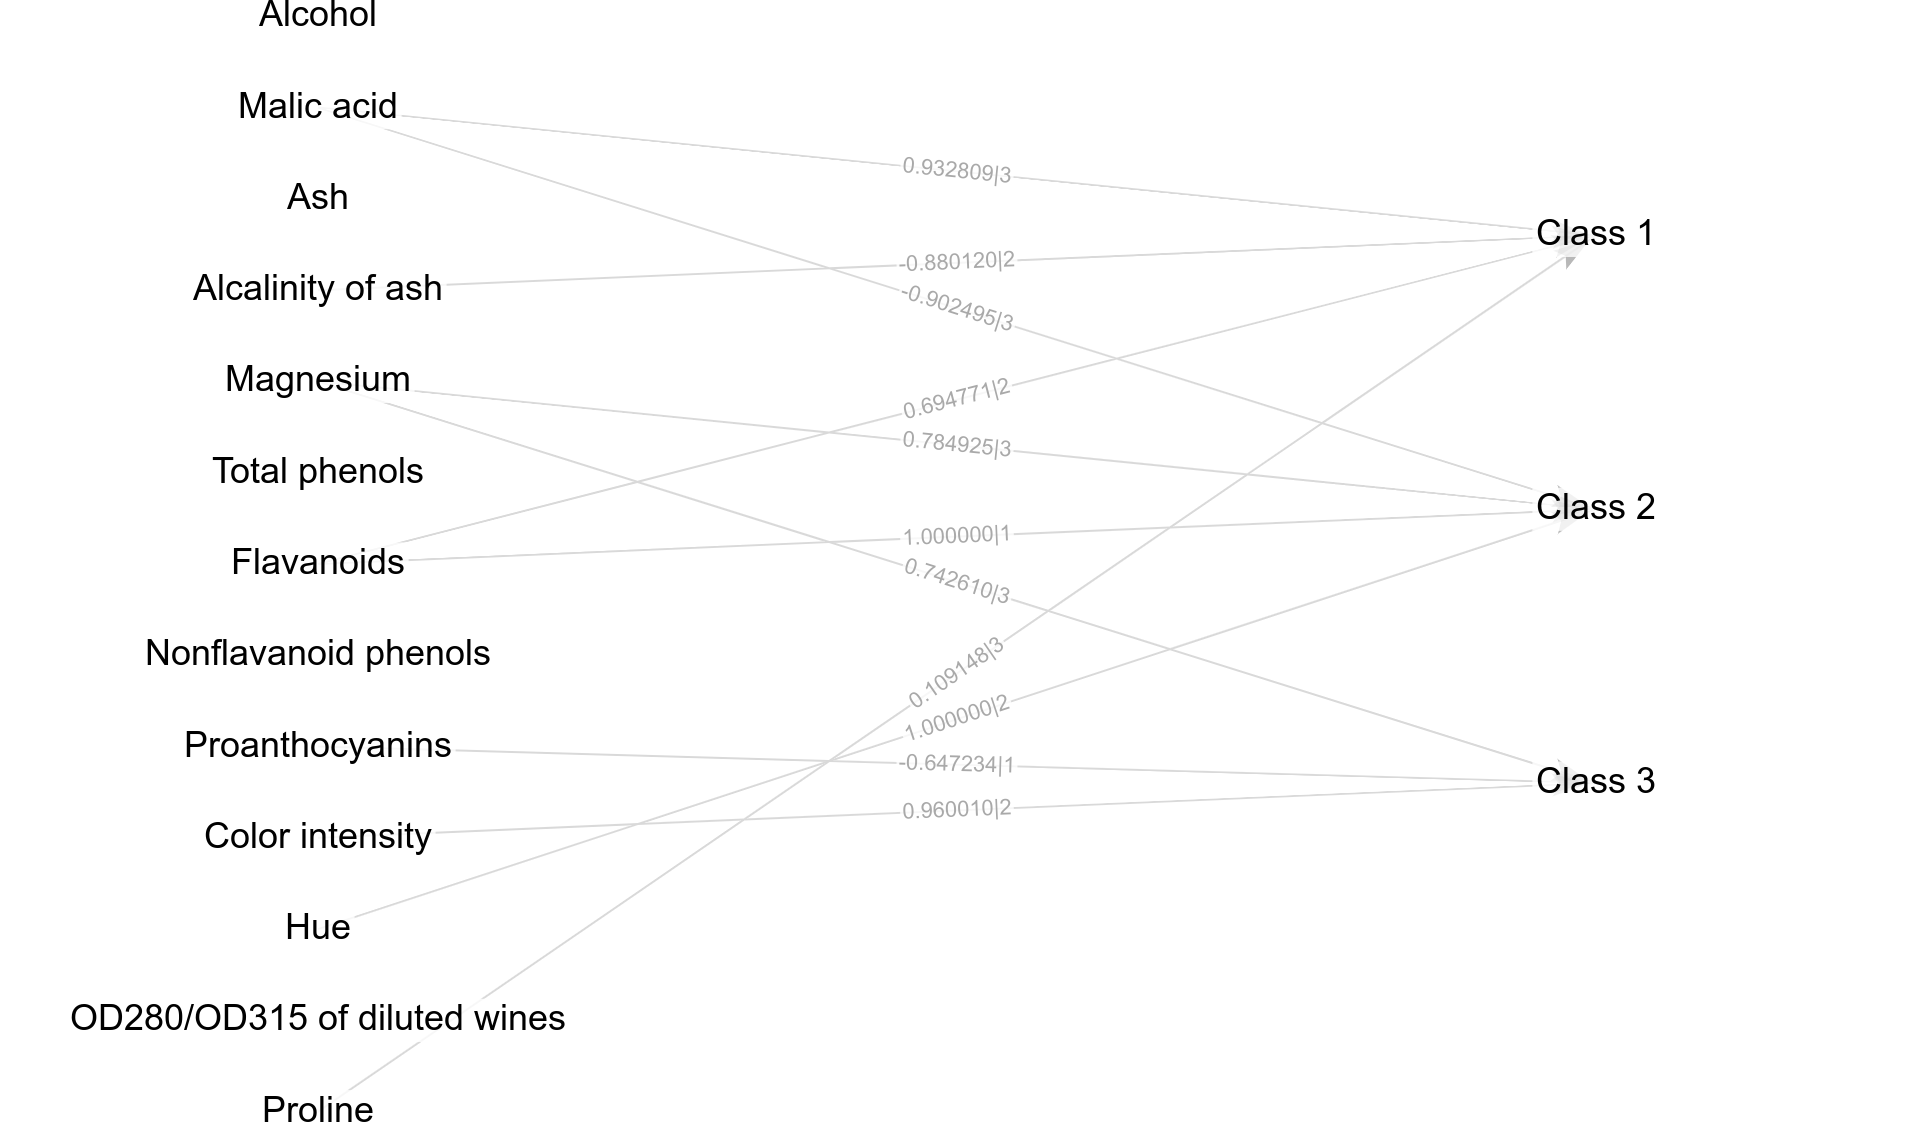
\includegraphics[width=13cm]{wine/2/mcc_g}
    \end{center}
    \caption{Vizualizacija agenta z največjim MCC drugega nabora. Vsebuje 1 globoko vozlišče in 7 povezav.}
    \label{fig:wine_mcc_2_g}
\end{figure}

\subsection{Tretji nabor}\label{subsec:dodatek-wine-tretji-nabor}
%%"/home/jure/CLionProjects/Neuroevolution/datasets/iris/iris.data" 350 25 75 4 true 0.1 175 true -0.001 -0.001 450 ACC
\begin{table}[H]
    \begin{center}
        \begin{tabular}{|| c | c c || c c ||}
            \hline
            \multirow{2}{*}{št. zagona} & \multicolumn{2}{c||}{točnost najboljšega agenta} & \multicolumn{2}{c||}{MCC najboljšega agenta} \\ \cline{2-5}
            & učna   & testna          & učna  & testna                  \\
            \hline
            1        & 80.0\% & 60.4\%          & 0.930 & 0.857                   \\
            \hline
            2        & 93.6\% & \textbf{96.2\%} & 0.906 & 0.860                   \\
            \hline
            3        & 95.2\% & 90.6\%          & 0.940 & 0.829                   \\
            \hline
            4        & 93.6\% & 88.7\%          & 0.774 & 0.763                   \\
            \hline
            5        & 88.0\% & 86.8\%          & 0.940 & \textbf{0.887 (92.5\%)} \\
            \hline
            $\sigma$ & 0.056  & 0.125           & 0.063 & 0.042                   \\
            \hline
        \end{tabular}
    \end{center}
    \caption{Rezultat tretjega nabora parametrov.}
    \label{tab:wine_result_3}
\end{table}

\begin{table}[H]
    \centering
    \begin{tabular}{||rcccc||}
        \hline
        razred  & Class 1 & Class 2 & Class 3 & vsota \\ \hline
        Class 1 & 18      & 0       & 0       & 18    \\ \hline
        Class 2 & 2       & 19      & 0       & 21    \\ \hline
        Class 3 & 0       & 0       & 14      & 14    \\ \hline
        vsota   & 20      & 19      & 14      & 53    \\ \hline
    \end{tabular}
    \caption{Matrika zmot najbolj točnega agenta tretjega nabora.}
    \label{tab:wine_acc_3}
\end{table}

\begin{table}[H]
    \centering
    \begin{tabular}{||rcccc||}
        \hline
        razred  & Class 1 & Class 2 & Class 3 & vsota \\ \hline
        Class 1 & 15      & 3       & 0       & 18    \\ \hline
        Class 2 & 1       & 20      & 0       & 21    \\ \hline
        Class 3 & 0       & 0       & 14      & 14    \\ \hline
        vsota   & 16      & 23      & 14      & 53    \\ \hline
    \end{tabular}
    \caption{Matrika zmot agenta z največjim MCC tretjega nabora.}
    \label{tab:wine_mcc_3}
\end{table}

\begin{figure}[H]
    \begin{center}
        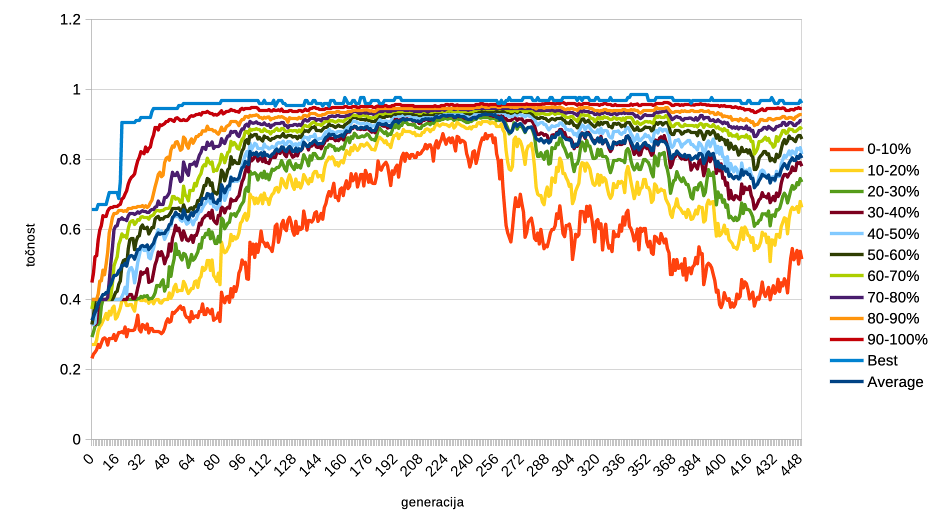
\includegraphics[width=13cm]{wine/3/acc}
    \end{center}
    \caption{Graf točnosti populacije najboljšega agenta tretjega nabora skozi generacije.}
    \label{fig:wine_acc_3}
\end{figure}

\begin{figure}[H]
    \begin{center}
        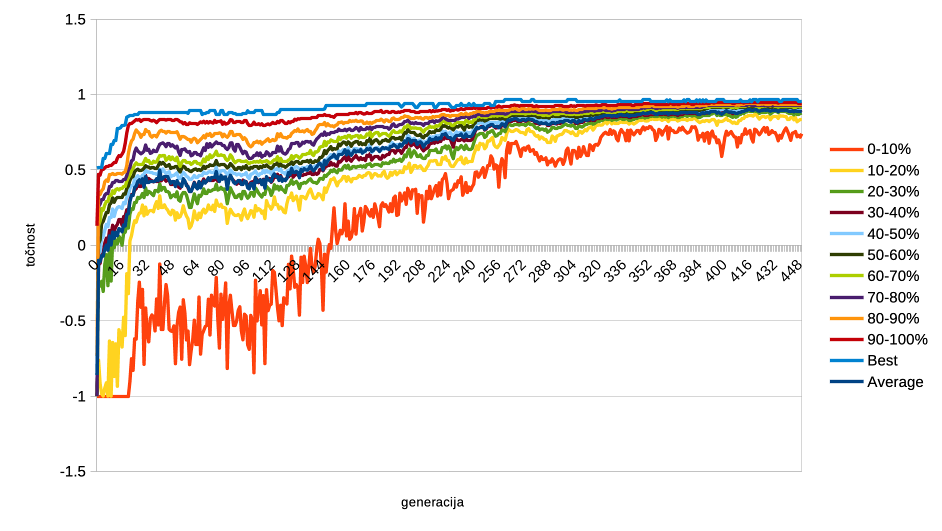
\includegraphics[width=13cm]{wine/3/mcc}
    \end{center}
    \caption{Graf MCC populacije najboljšega agenta tretjega nabora skozi generacije.}
    \label{fig:wine_mcc_3}
\end{figure}

\begin{figure}[H]
    \begin{center}
        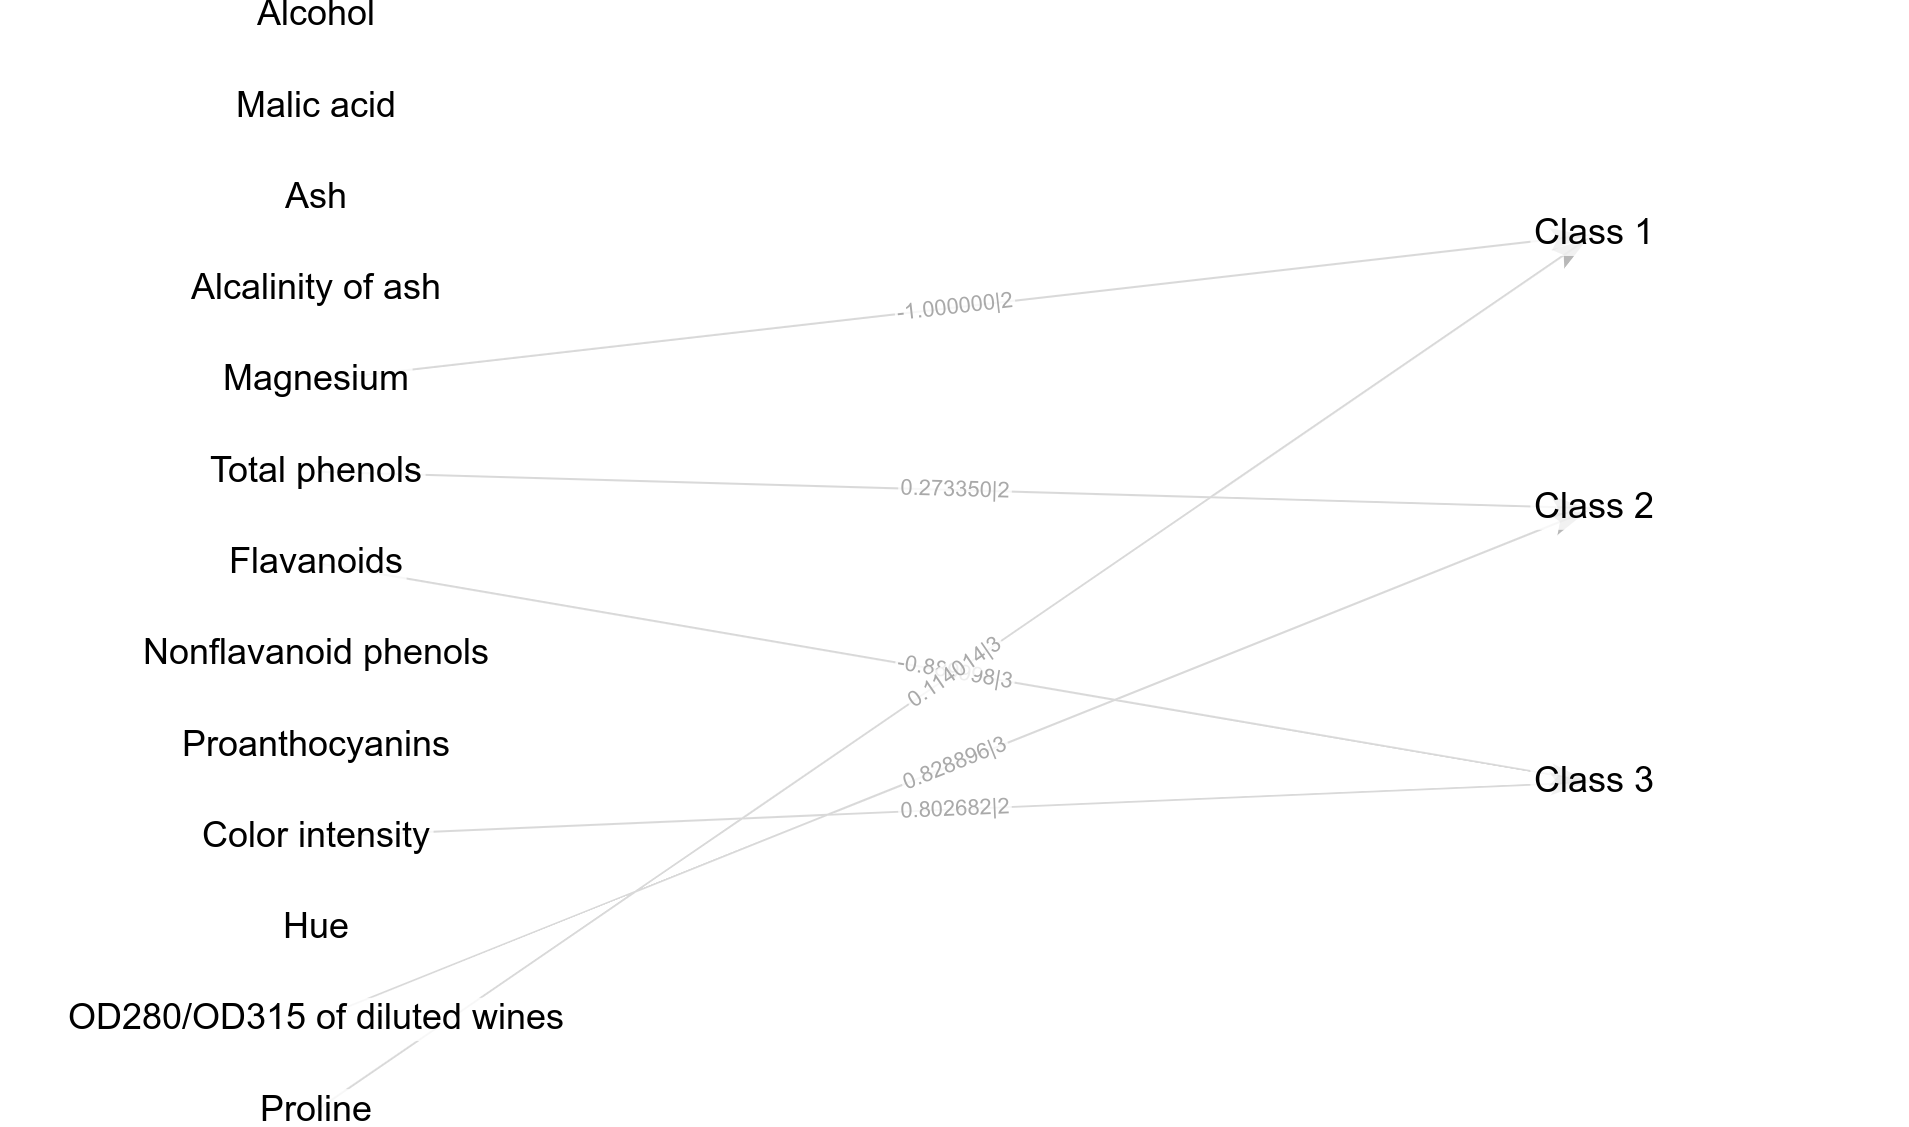
\includegraphics[width=13cm]{wine/3/acc_g}
    \end{center}
    \caption{Vizualizacija najbolj točnega agenta tretjega nabora. Vsebuje 11 povezav.}
    \label{fig:wine_acc_3_g}
\end{figure}

\begin{figure}[H]
    \begin{center}
        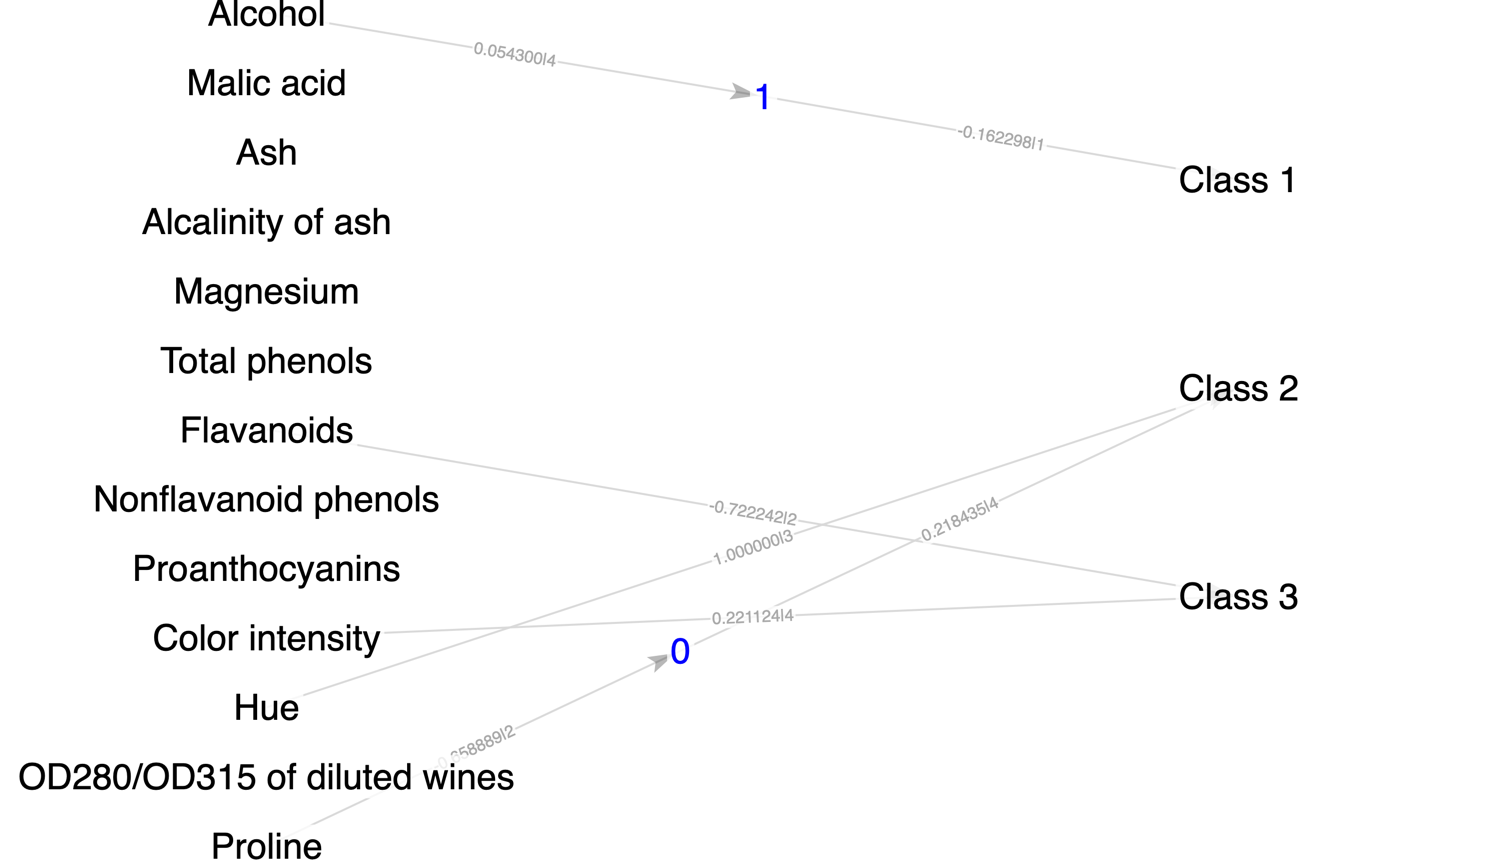
\includegraphics[width=13cm]{wine/3/mcc_g}
    \end{center}
    \caption{Vizualizacija agenta z največjim MCC tretjega nabora. Vsebuje 2 globoki vozlišči in 7 povezav.}
    \label{fig:wine_mcc_3_g}
\end{figure}